\documentclass[11pt]{beamer}
%\setbeameroption{show notes}
\usetheme{CambridgeUS}
\usepackage[utf8]{inputenc}
\usepackage[german]{babel}
\usepackage{amsmath}
\usepackage{amsfonts}
\usepackage{amssymb}
\usepackage{url}
\usepackage{multimedia}
%\pgfpageuselayout{4 0n 1 with notes}[a4paper,border shrink=5mm]
\usepackage{color}
\definecolor{mygreen}{rgb}{0,0.6,0}
\definecolor{mygray}{rgb}{0.5,0.5,0.5}
\usepackage{listings}
\usepackage{outlines}
% https://en.wikibooks.org/wiki/LaTeX/Source_Code_Listings
% http://texblog.org/2012/08/29/changing-the-font-size-in-latex/
\lstset{basicstyle=\scriptsize 
        , commentstyle=\color{mygreen}
        , keywordstyle=\color{blue}
        , language=C++
        %, frame=single
    }

\author{Richard Ulrich}
\title{Docker}
\subtitle{An introduction to docker containers}
\setbeamercovered{dynamic} 
\institute{BORM Informatik AG} 
%\date{} 
\subject{BORM developer day} 
\titlegraphic{
\includegraphics[width=2cm]{borm_logo.jpg}}

\begin{document}

%%%%%%%%%%%%%%%%%%%%%%%%%%%%%%%%%%%%%%%%%%%%%%%%%%%%%%%%%%%%%%%%%%%%%%%%%%%%%%%
\begin{frame}
\titlepage
\end{frame}

%%%%%%%%%%%%%%%%%%%%%%%%%%%%%%%%%%%%%%%%%%%%%%%%%%%%%%%%%%%%%%%%%%%%%%%%%%%%%%%
\begin{frame}{Why ``works on my machine'' is not enough}
\textbf{Releasing binaries reproducibly}
\begin{itemize}
\item there was a time, when the release compiled binary from a developers machine was shipped to the customers
\item these days we only ship binaries from bamboo
\item we track revisions and dependencies
\item but the configuration of the build agents became complicated over time
\item docker offers a way to define the environment in a text file
\item the docker file can be versioned
\end{itemize}
\end{frame}

%%%%%%%%%%%%%%%%%%%%%%%%%%%%%%%%%%%%%%%%%%%%%%%%%%%%%%%%%%%%%%%%%%%%%%%%%%%%%%%
\begin{frame}{Table of contents}
\begin{itemize}
\item Introduction video
\item Dissection of an example
\end{itemize}
\end{frame}

%%%%%%%%%%%%%%%%%%%%%%%%%%%%%%%%%%%%%%%%%%%%%%%%%%%%%%%%%%%%%%%%%%%%%%%%%%%%%%%
\begin{frame}{Introduction video}
%https://tex.stackexchange.com/questions/89088/how-to-embed-video-and-animation-in-latex-and-latex-beamer-step-by-step
\centering
\movie[label=show3,width=1.0\textwidth,poster
       ,autostart,showcontrols,loop] 
  {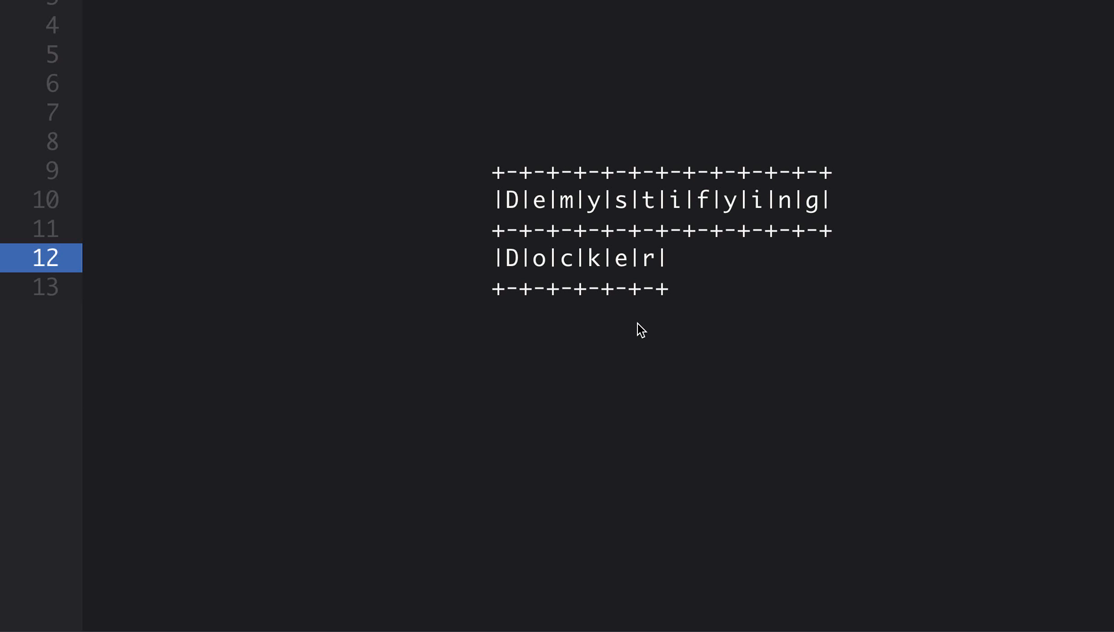
\includegraphics[width=1.0\textwidth]{pGYAg7TMmp0.png}}{pGYAg7TMmp0.webm}
\end{frame}

%%%%%%%%%%%%%%%%%%%%%%%%%%%%%%%%%%%%%%%%%%%%%%%%%%%%%%%%%%%%%%%%%%%%%%%%%%%%%%%
\begin{frame}{Dissection of an example}
\begin{outline}
\1 Jaxx is a multi cryptocurrency wallet
\1 Unfortunately it is available only as closed source
\1 Risks include:
  \2 Stealing of private keys stored on the harddisk
  \2 Exposing transaction history from stored wallets
\1 Docker offers protection by running in an encapsulated environment
\1 Much more lightweight and convenient than a virtual machine
\end{outline}
\end{frame}

%%%%%%%%%%%%%%%%%%%%%%%%%%%%%%%%%%%%%%%%%%%%%%%%%%%%%%%%%%%%%%%%%%%%%%%%%%%%%%% 
\begin{frame}{Dockerfile - Defining the base environment} 
\lstinputlisting[language=bash, firstline=0, lastline=16]{@docker_SOURCE_DIR@/Dockerfile}
\end{frame}

%%%%%%%%%%%%%%%%%%%%%%%%%%%%%%%%%%%%%%%%%%%%%%%%%%%%%%%%%%%%%%%%%%%%%%%%%%%%%%% 
\begin{frame}{Dockerfile - Download and unpack binary} 
\lstinputlisting[language=bash, firstline=17, lastline=21]{@docker_SOURCE_DIR@/Dockerfile}
\end{frame}

%%%%%%%%%%%%%%%%%%%%%%%%%%%%%%%%%%%%%%%%%%%%%%%%%%%%%%%%%%%%%%%%%%%%%%%%%%%%%%% 
\begin{frame}{Dockerfile - Determine and satisfy dependencies} 
\lstinputlisting[language=bash, firstline=23, lastline=33]{@docker_SOURCE_DIR@/Dockerfile}
\end{frame}

%%%%%%%%%%%%%%%%%%%%%%%%%%%%%%%%%%%%%%%%%%%%%%%%%%%%%%%%%%%%%%%%%%%%%%%%%%%%%%% 
\begin{frame}{Dockerfile - Set up user environment} 
\lstinputlisting[language=bash, firstline=35, lastline=49]{@docker_SOURCE_DIR@/Dockerfile}
\end{frame}

%%%%%%%%%%%%%%%%%%%%%%%%%%%%%%%%%%%%%%%%%%%%%%%%%%%%%%%%%%%%%%%%%%%%%%%%%%%%%%% 
\begin{frame}{Dockerfile - Entry point} 
\lstinputlisting[language=bash, firstline=51, lastline=52]{@docker_SOURCE_DIR@/Dockerfile}
\end{frame}

%%%%%%%%%%%%%%%%%%%%%%%%%%%%%%%%%%%%%%%%%%%%%%%%%%%%%%%%%%%%%%%%%%%%%%%%%%%%%%% 
\begin{frame}{Execution} 
Build the docker container, and execute the bundled application
\lstinputlisting[language=bash]{@docker_SOURCE_DIR@/jaxx.sh}
\end{frame}

%%%%%%%%%%%%%%%%%%%%%%%%%%%%%%%%%%%%%%%%%%%%%%%%%%%%%%%%%%%%%%%%%%%%%%%%%%%%%%% 
\begin{frame}{Docker on Windows} 
\begin{itemize}
\item Same principle as on linux
\item More complicated to install stuff
\item See for yourself: \url{https://blogs.msdn.microsoft.com/heaths/2017/09/18/installing-build-tools-for-visual-studio-2017-in-a-docker-container/}
\end{itemize}
\end{frame}

%%%%%%%%%%%%%%%%%%%%%%%%%%%%%%%%%%%%%%%%%%%%%%%%%%%%%%%%%%%%%%%%%%%%%%%%%%%%%%%
\begin{frame}{Closing}
All code presented in this document can be found at:\\
\url{https://github.com/ulrichard/experiments/tree/master/docker}\\
-\\
It was written using vim, LaTeX and cmake. For more details see:\\
\url{http://blog.ulrichard.ch/?p=1406}\\
-\\
Thanks for listening
-\\
Do you have questions?
\end{frame}

\end{document}

